\documentclass[revtex4-2]{mpltx}

\begin{document}
\title{非线性对流斑图}
\author{方尤乐}

\emailphone{eden@stu.pku.edu.cn}{(86)15313960363}
\affiliation{北京大学物理学院\quad 学号: 2000012416}
\begin{abstract}
    贝纳对流现象与非线性动力学有关,是研究耗散结构理论的重要系统。
    本实验通过控制 2mm 和 4mm 薄层去离子水的上表面下表面温度差,通过阴影法,观察非线性对流斑图从无到有的涌现,
    而后从稳定到失稳湍流的过程,并借助图像定性地分析了系统相应结构的特征。
\end{abstract}
\keywords{对流斑图、耗散结构、贝纳对流、非线性动力学}
\maketitle
\section{引言}
自然界和人们的生活中充斥着不可逆过程,但科学地研究这样的过程却姗姗来迟。19世纪克劳修斯等人提出热力学第二定律,指出孤立系统的熵永不减小,
最终将达到极大值,即热力学的平衡态。然而自然界存在着丰富的自组织现象,由局域的相互作用、从无序初态出发,自发地产生出更大尺度上的有序结构。
例如结晶过程(如冰晶形成),化学振荡(如碘钟),生命过程(如进化,蛋白质的合成与折叠)等等,这些现象与热力学第二定律暗示的无序演化相反。
基于此,普利高津于上世纪 60 年代发展出了耗散结构理论,并于 1977 年获得诺贝尔化学奖。\cite{jindaishiyan}

耗散结构理论表明,当开放系统偏离平衡达一定程度时,系统将会出现分岔行为,此后系统将离开原先无序的热力学分支,发生突变进入到一个全新的稳定有
序状态,即耗散结构。本实验观察的贝纳对流正是耗散结构的一个具体实例。

\section{实验装置}
实验装置如图所示。本实验观察 d = 2 mm, 4 mm 的对流层,
上、下表面均选用高热导率界面以使温度均匀分布。
上表面水冷降温,采用透明介质以便于观察;
底面为硅胶片加热的铜盘,表面光洁作为反射面。

本实验通过阴影法观察对流斑图,用准平行光正入射液层,
考察经底面铜盘反射的光线之光强分布。
光强分布直接反映液层的折射率分布;由费马原理,光线向高
折射率区域偏折,高折射率区域将会聚光线而形成亮区。
所以高折射率对应高密度,即对流中的冷水下降区域。
\begin{figure}[htbp]
    \centering
    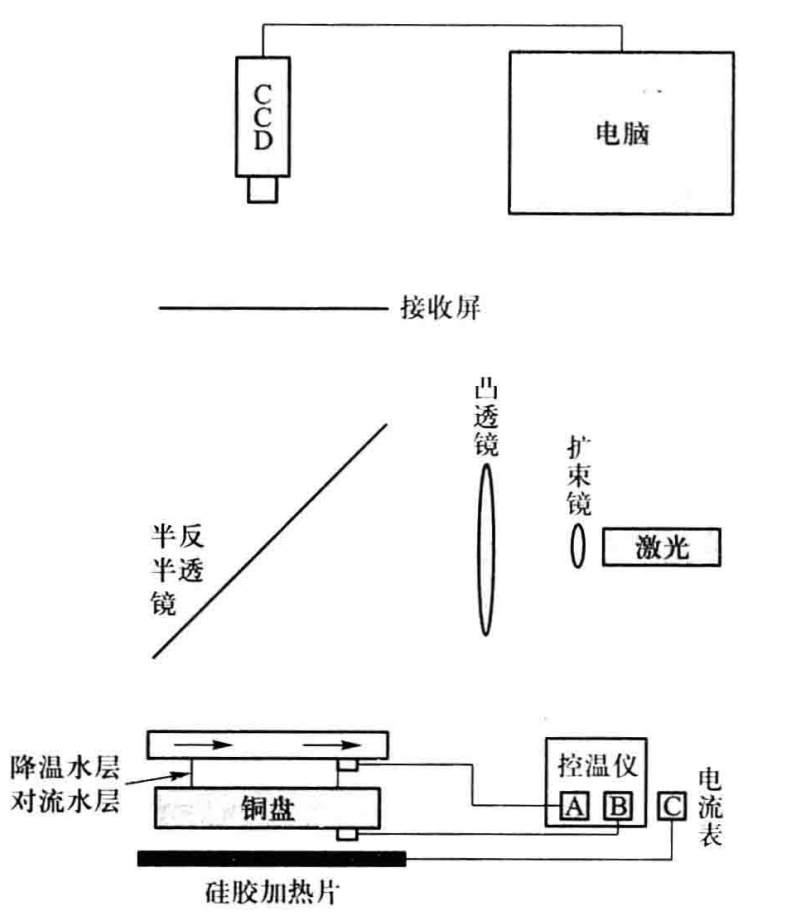
\includegraphics[width=0.6\textwidth]{1.png}
    \caption{实验装置示意图}
    \label{fig:1}
\end{figure}
\section{结果和讨论}
实验中由加热电流控制温差 $\Delta T$, 调整加热电流后等待 10 min $\sim$ 20 min 使系统
达到稳恒态。室温条件下测得上表面温度与下表面温度不相同,此时的上下表面温差可能来自于电路接触点的电阻,
因此需要减去 $\Delta T$ 得到真实的温差。

\begin{figure}[htbp]
    \centering
    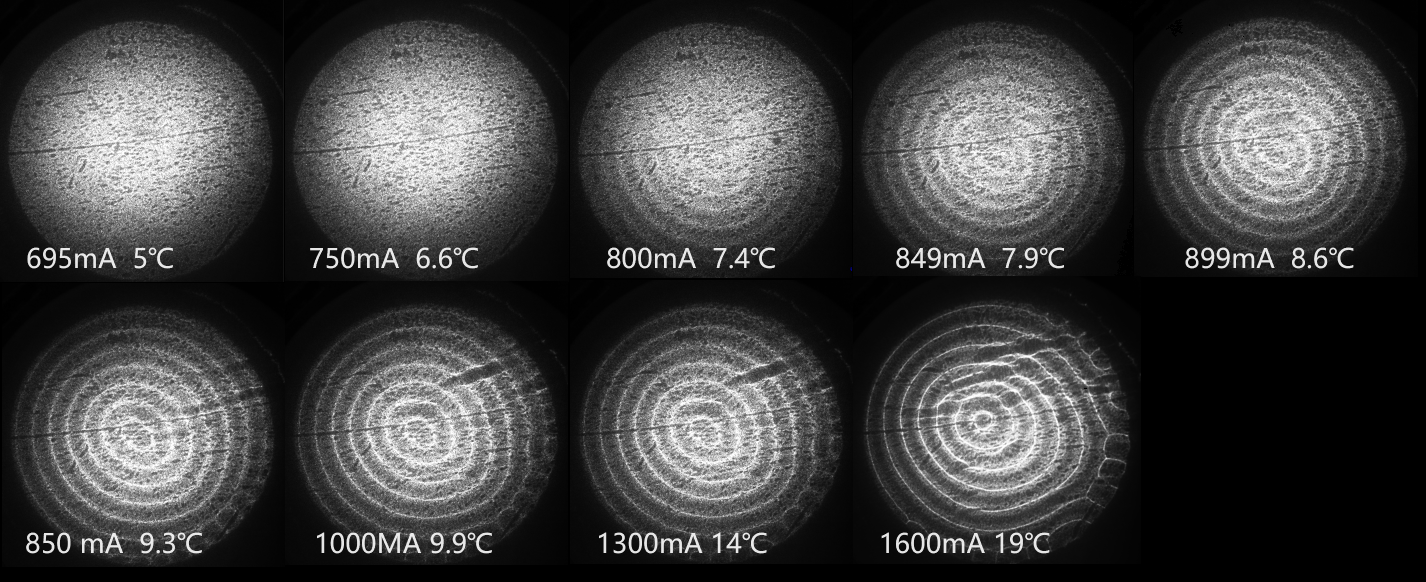
\includegraphics[width=0.9\textwidth]{2.png}
    \caption{2 mm 薄层的对流斑图}
    \label{fig:2}
\end{figure}
\begin{figure}[htbp]
    \centering
    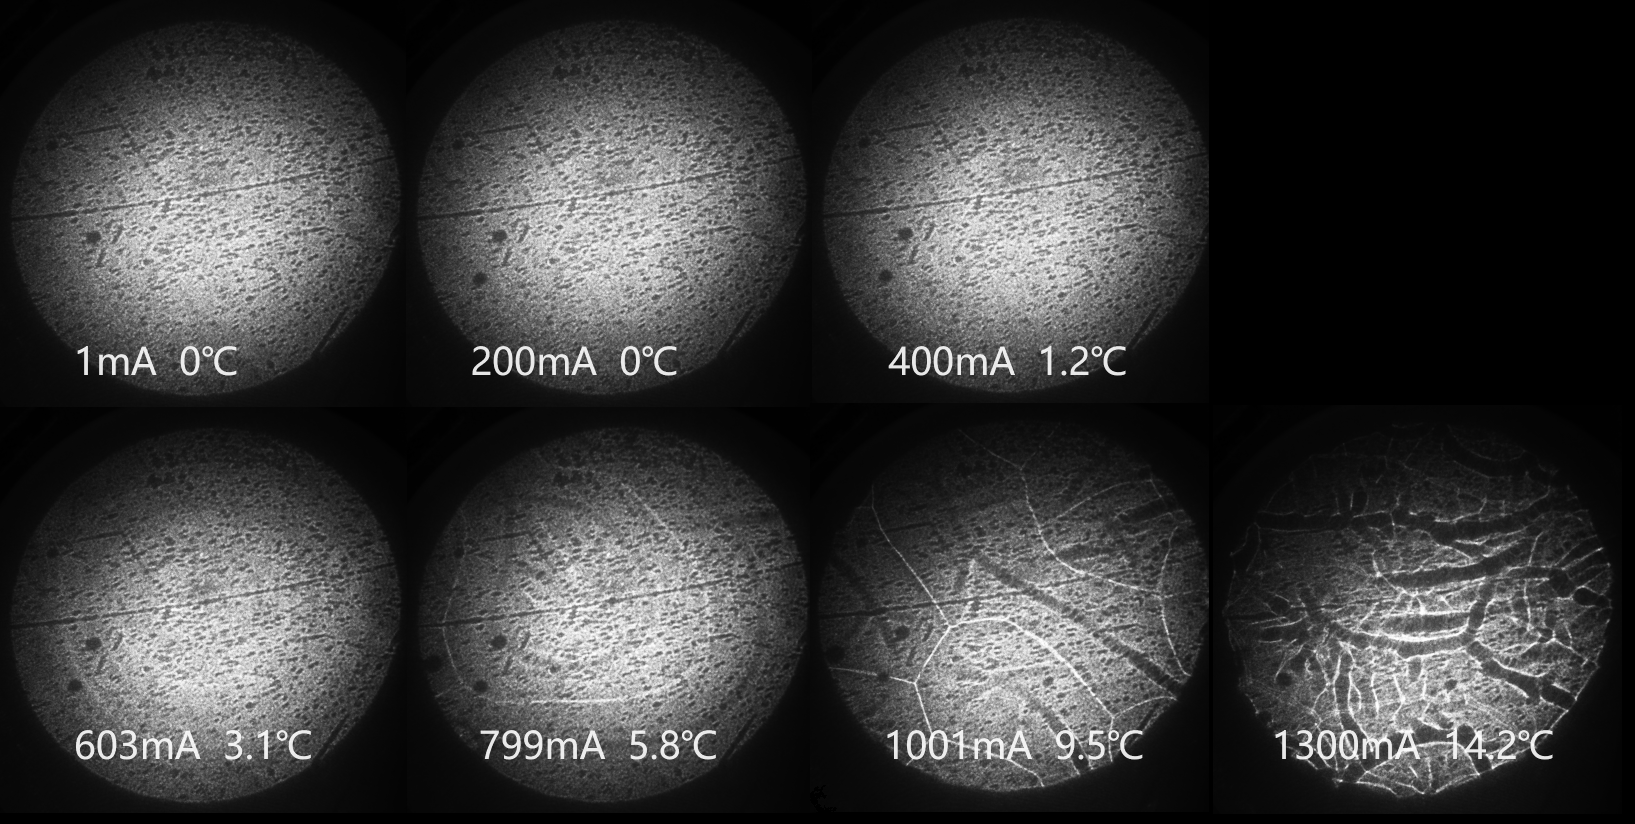
\includegraphics[width=0.9\textwidth]{3.png}
    \caption{4 mm 薄层的对流斑图}
    \label{fig:3}
\end{figure}

实验结果如图 \ref{fig:2} 和 \ref{fig:3} 所示,每张图的左下角有标注加热电流的大小和上下表面的实际温差。
可以看到,当温差较小时,没有对流斑图,图像中没有明显特征。
当温差过一个临界值后,对流斑图开始出现,且斑图的对比度随温差的增大而增强。
对于 2 mm 薄层,温差的临界值约为 7 $^\circ$C; 4 mm 薄层,温差的临界值约为 3 $^\circ$C。
出现斑图的临界温差降低,是因为 4 mm 薄层在 $z$ 方向上的范围增大,由瑞利数 $Ra\propto d^3\Delta T$ 和临界条件 $Ra=R_c$,
所以临界温差降低为原来的 $1/8$ 倍。实验观察得到的临界温差降低程度不如 $1/8$ 那么显著,可能是由于上述的理论计算是在无限大平面条件下做的计算,
和实验条件中有限大圆盘的情况有所不同。此外,4 mm 薄层的斑图原胞比 2 mm 的对流斑图元胞的尺度更大,耗散结构破坏也出现得更糟。
如 \ref{fig:3} 中最后两张图中,大元胞裂解为小元胞以维持耗散结构的稳定性。预计继续升温,斑图会彻底崩溃出现不断变换的湍流。
\section{结论}
本实验通过考察耗散结构的经典实例:贝纳对流斑图;实验中比较了 d = 2 mm, 4 mm 薄层去离子水的上下表面温差,观察分析了斑图从无到有至破坏的过程,
认识并检验了耗散结构的基本特征,对耗散结构理论有了更直观的理解。
\begin{acknowledgments}
    感谢周路群老师的细致指导,尤其是老师关于耗散结构和非线性动力学的讲解对
本人带来了很大启发;感谢合作者汪奕程同学的工作和帮助。
\end{acknowledgments}
\begin{thebibliography}{99}
    \bibitem{jindaishiyan} 吴思诚、荀坤. 近代实验物理[M]. 高等教育出版社, 2015.
\end{thebibliography}
\clearpage
\appendix
\section{思考题}
\subsection{随着温差的升高,可看到黑白结构的出现,黑白区域如何对应水层的流动情况?}
黑白结构的出现是由于水层中形成稳定有序的流动。
黑色区域对应着水层中的上升流,白色区域对应着水层中的下降流。
因为下降流密度较大,折射率较高,光线被聚焦,所以看起来比较亮;
黑色区域的密度较小,折射率较低,光线被发散,所以看起来比较暗。

\subsection{斑图出现的临界点如何确定?如何根据所观察到的现象确定临界点?}
实验通过加热电流控制温差,逐步增大温差,当能观察到略微的明暗交替,稳定的元胞出现后,可以确定斑图出现。
此时对比度较小是因为斑图明暗区域之间的对流较弱,上升流和下降流的密度差异不大,所以折射率差异不大,对比度较低。

\subsection{当水层换成 4 mm 时,考虑临界点会如何改变?并注意实验过程中参数的选择。}
临界点会变小,是因为 4 mm 薄层在 $z$ 方向上的范围增大,由瑞利数 $Ra\propto d^3\Delta T$ 和临界条件 $Ra=R_c$,
所以临界温差降低为原来的 $1/8$ 倍。实验观察得到的临界温差降低程度不如 $1/8$ 那么显著,可能是由于上述的理论计算是在无限大平面条件下做的计算,
和实验条件中有限大圆盘的情况有所不同。
\subsection{如何确定斑图的空间特征尺度?}
测量斑图中相邻两条亮条纹之间的垂直距离。
\subsection{斑图的空间特征尺度与对流水层厚度的关系如何?}
斑图水平尺度大致正比于对流水层厚度 $d$,这可以由 \cite{jindaishiyan} 中的稳定解公式得到。
\end{document}